%%%%%%%%%%%%%%%%%%%%%%%%%%%%%%%%%%%%%%%%%
% A beamer poster style for the University of Oxford. Atilim Gunes Baydin <gunes@robots.ox.ac.uk>, November 2016.
% Based on the I6pd2 style created by Thomas Deselaers an Philippe Dreuw.
%
% Dreuw & Deselaer's Poster
% LaTeX Template
% Version 1.0 (11/04/13)
%
% Created by:
% Philippe Dreuw and Thomas Deselaers
% http://www-i6.informatik.rwth-aachen.de/~dreuw/latexbeamerposter.php
%
% This template has been downloaded from:
% http://www.LaTeXTemplates.com
%
% License:
% CC BY-NC-SA 3.0 (http://creativecommons.org/licenses/by-nc-sa/3.0/)
%
%%%%%%%%%%%%%%%%%%%%%%%%%%%%%%%%%%%%%%%%%

%----------------------------------------------------------------------------------------
%   PACKAGES AND OTHER DOCUMENT CONFIGURATIONS
%----------------------------------------------------------------------------------------

\documentclass[final,hyperref={pdfpagelabels=false}]{beamer}

\usepackage[orientation=portrait,size=a1,scale=1.43]{beamerposter} % Use the beamerposter package for laying out the poster with a portrait orientation and an a0 paper size

\usetheme{Oxford}

\usepackage[utf8]{inputenc} % allow utf-8 input
\usepackage{blindtext}
\usepackage{ragged2e}
\usepackage{amsmath,amsthm,amssymb,latexsym} % For including math equations, theorems, symbols, etc
\usepackage{ragged2e}
\usepackage{times}\usefonttheme{professionalfonts}  % Uncomment to use Times as the main font
\usefonttheme[onlymath]{serif} % Uncomment to use a Serif font within math environments
%\boldmath % Use bold for everything within the math environment
\usepackage{booktabs} % Top and bottom rules for tables
\usepackage{microtype}
\usepackage{subcaption}
\usepackage{tikz}
\usepackage{pgfplots}
\usepackage{svg}

\usetikzlibrary{positioning, shapes, arrows.meta}



\usecaptiontemplate{\small\structure{\insertcaptionname~\insertcaptionnumber: }\insertcaption} % A fix for figure numbering

\newcommand{\shrink}{-15pt}

\def\imagetop#1{\vtop{\null\hbox{#1}}}

\let\oldbibliography\thebibliography
\renewcommand{\thebibliography}[1]{\oldbibliography{#1}
\setlength{\itemsep}{-10pt}}

%----------------------------------------------------------------------------------------
%   TITLE SECTION 
%----------------------------------------------------------------------------------------
\title{{\Huge Large Agent Collider}\vspace{0.3cm}\\ Studying complexity with agent-based models}
\author{Nicholas Bishop, Joel Dyer, Imran Hashmi, Arnau Quera-Bofarull, Hao Zhou, \\ Anisoara Calinescu, Doyne Farmer, Michael Wooldridge}
\institute{Department of Computer Science, University of Oxford\\\vspace{4mm}
\texttt{\{name.surname\}@cs.ox.ac.uk}}

%----------------------------------------------------------------------------------------
%   FOOTER TEXT
%----------------------------------------------------------------------------------------
\newcommand{\leftfoot}{} % Left footer text
\newcommand{\rightfoot}{} % Right footer text


%----------------------------------------------------------------------------------------

\begin{document}
\addtobeamertemplate{block end}{}{\vspace*{2ex}} % White space under blocks

\begin{frame}[t] % The whole poster is enclosed in one beamer frame

\begin{columns}[t] % The whole poster consists of three major columns, each of which can be subdivided further with another \begin{columns} block - the [t] argument aligns each column's content to the top

  \begin{column}{.02\textwidth}\end{column} % Empty spacer column

%%%%%%%%%%%%%%%%%%%%%%%%%%%%%%%%%%%%%%%%%%
%% Column 1
%%%%%%%%%%%%%%%%%%%%%%%%%%%%%%%%%%%%%%%%%%

  \begin{column}{.48\textwidth} % 1st column

    \vspace{\shrink}          
    \begin{block}{1. Agent-Based Models}
      \begin{itemize}
          \item Agent-based modelling (\textbf{ABMing}) is a simulation technique to study complex systems.
          \item In ABMing, we simulate the actions and interactions of autonomous agents in order to understand the emerging collective behaviour of the system.
          \item Agent-based models (\textbf{ABMs}) are used in many fields, including biology, economics, and sociology.
      \end{itemize}
      \begin{figure}
        \centering
        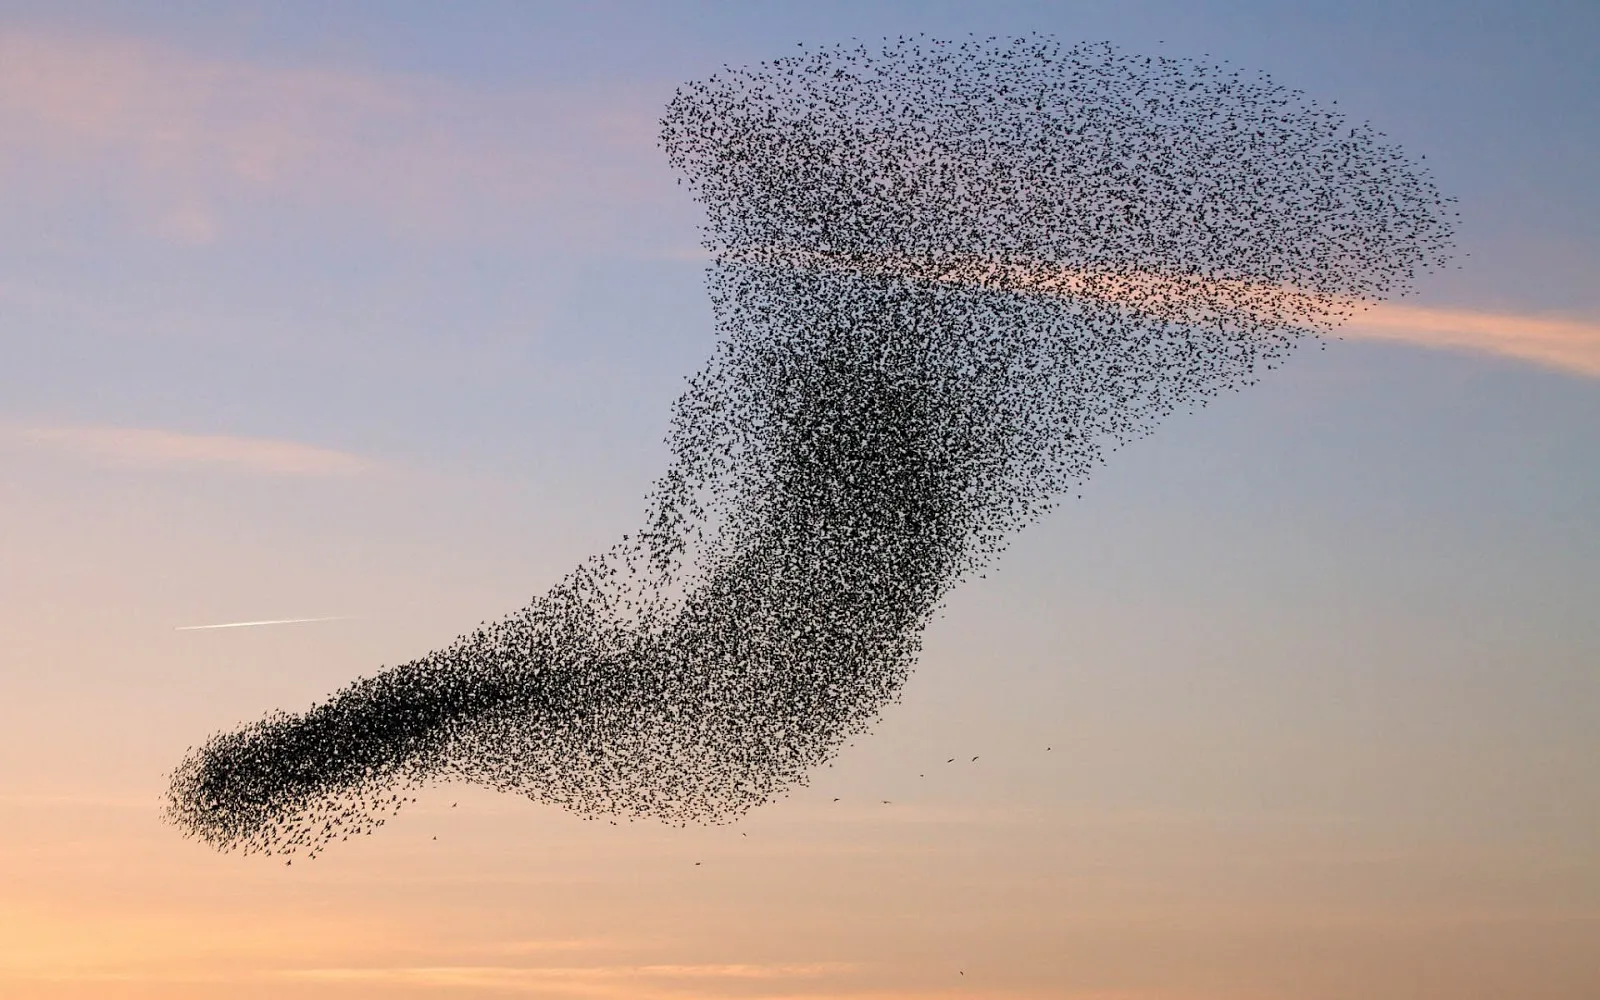
\includegraphics[width=0.8\columnwidth]{figures/birds}
        \caption{\footnotesize The flocking of a pack of birds is an emergent feature of the bird's individual behaviour.}
      \end{figure}
    \end{block}
    \begin{block}{3. Challenges of Agent-Based Modelling}
      The effective use of ABMs in wider settings such as policy making is hindered by:
      \begin{itemize}
        \item\justifying \textbf{A. Expensive to simulate}: ABMs involve simulating potentially millions of agents, which is computationally expensive.
        \item\justifying \textbf{B. Data availability:} The granularity of ABMs requires a lot of data, which is often not available.
        \item\justifying\textbf{C. Tough to calibrate}: ABMs are often used to make predictions about the real world, but it is difficult to validate the truthfulness of the model.
        \item\justifying \textbf{D. Difficult to analyse}: The complexity of ABMs makes it difficult to understand the causal 
          relationships between the agents and the emergent behaviour of the system.
        \item\justifying \textbf{E. Hard to reproduce}: Programming ABMs is difficult, and it is often hard to 
          reproduce the results of a model done by another researcher.
      \end{itemize}
    \end{block}

  \end{column} % End of the 1st column

%%%%%%%%%%%%%%%%%%%%%%%%%%%%%%%%%%%%%%%%%%
%% Column 2
%%%%%%%%%%%%%%%%%%%%%%%%%%%%%%%%%%%%%%%%%%

  \begin{column}{.02\textwidth}\end{column} % Empty spacer column

  \begin{column}{.48\textwidth} % 2nd column
    \vspace{\shrink}
    \begin{block}{2. Example : Epidemiology}
      \begin{itemize}
        \item We can study the spread of a disease in a population using an ABM.
        \item We do so by simulating the movement and interactions of individuals in a population.
        \item A good example is the agent-based SIR (Susceptible, Infectious, Recovered) model, where disease can spread after a contact with an infectious individual.
        \vspace{1cm}
          \begin{figure}
            \captionsetup[subfigure]{justification=centering}
            \begin{subfigure}[t]{0.3 \columnwidth}
              \begin{tikzpicture}[node distance=3cm,>=Stealth,auto, scale=1.2]
      
                % Define person node
                %\tikzstyle{person} = [circle, draw, fill=blue!20, minimum size=20pt, inner sep=0pt]
                \tikzstyle{person} = [path picture={\node at (path picture bounding box.center) {
\includegraphics[width=20pt]{figures/person}};}]
      
      
                % Create 10 person nodes with more spaced positions
                \foreach \i/\x/\y in {1/0/0, 2/2/0, 3/-1/2, 4/1/2, 5/3/2, 6/3/4, 7/-0.2/4, 8/-1/6.5, 9/1/6, 10/-1/3}
                    \node[person] (p\i) at (\x, \y) {};
      
                % Draw connections to resemble clusters
                \foreach \i in {1,...,4}
                    \foreach \j in {\i,...,5}
                        \draw (p\i) -- (p\j);
      
                \foreach \i in {6,...,8}
                    \foreach \j in {\i,...,10}
                        \draw (p\i) -- (p\j);
      
                \draw (p4) -- (p6);
              \end{tikzpicture}
              \caption{\footnotesize Graph representing the contacts of the population.}
            \end{subfigure}
            \begin{subfigure}[t]{0.5 \columnwidth}
              \begin{tikzpicture}[scale=1.25 ]
                \begin{axis}[
                  xlabel={Time [ days ]},
                  ylabel={Population [\%]},
                  legend pos=north west,
                  legend style={font=\footnotesize}, 
                  grid=both,
                  axis lines=left,
                  xlabel style={font=\scriptsize},
                  ylabel style={font=\scriptsize},
                  tick label style={font=\scriptsize}
                ]
                  \addplot[domain=0:10, smooth, ultra thick, blue] {50 * (1 - 1 / (1 + exp(-0.5 * (x - 5))))};
                  \addlegendentry{Susceptible};

                  \addplot[domain=0:10, smooth, ultra thick, red] {100 / (1 + exp(-0.5 * (x - 5)))};
                  \addlegendentry{Infectious};

                  \addplot[domain=0:10, smooth, ultra thick, green] {50 / (1 + exp(-0.5 * (x - 5)))};
                  \addlegendentry{Recovered};
                \end{axis}
              \end{tikzpicture}
              \caption{\footnotesize Percentage of the population in each state over time.}
            \end{subfigure}
          \end{figure}
      \vspace{0.5cm}
      \item The spread of the disease will depend on multiple factors, including the behaviour and contact patterns of individuals.
      \end{itemize}
    \end{block}


    \begin{block}{4. How are we tackling these challenges?}
      In our research group, we are tackling these challenges using the following techniques:
      \begin{itemize}
        \item \justifying \textbf{A. Tensorized simulation}: By leveraging modern software for tensorized computation, we can simulate ABMs orders of magnitude faster than traditional implementations.
        \item \justifying \textbf{B. Scenario-generation}: When fine-grained data not available, we can use ABMs as a scenario-based planning tool to help policy making under uncertainty.
        \item \justifying \textbf{C. Differentiable programming}: We can use automatic differentiation to enable gradient-based calibration of ABMs.
        \item \justifying \textbf{D. Causal inference}: Causal inference techniques can help us understand the causal relationships between the agents and the emergent behaviour of the system.
        \item \justifying \textbf{E. Open-source software}: All our research software is open-source, and we use modern software engineering practices to ensure reproducibility.

      \end{itemize}
    \end{block}

  \end{column} % End of the 2nd column

%%%%%%%%%%%%%%%%%%%%%%%%%%%%%%%%%%%%%%%%%%
%% Column 3
%%%%%%%%%%%%%%%%%%%%%%%%%%%%%%%%%%%%%%%%%%


  \begin{column}{.02\textwidth}\end{column} % Empty spacer column

\end{columns} % End of all the columns in the poster

\begin{minipage}{\textwidth}
  \begin{block}{5. Results and Impact}
    \begin{itemize}
      \item We have dramatically accelerated the simulation, calibration, and analysis of ABMs involving millions of agents in epidemiological and financial domains \cite{10.5555/3545946.3598851, 10.1145/3604237.3626857, 10.5555/3545946.3598853, bayesian_diff, some_challenges}.
      \item We have developed an open-source package for the Bayesian calibration of differentiable simulators using the developed techniques \cite{blackbirds}.
      \item We have developed a novel methodology for scenario-generation based planning under uncertainty using ABMs \cite{synthpop}.
      \item We have adapted secure multi-party computation techniques to enable privacy-preserving simulation, calibration, and analysis of ABMs \cite{decabm}.
      \item TODO: Causal stuff?
  \end{itemize}
  \end{block}
  \begin{block}{Bibliography}
    %\nocite{*} % Insert publications even if they are not cited in the poster
    \linespread{0.928}\selectfont
    \scriptsize{\bibliographystyle{abbrv}\bibliography{lac_papers}}
  \end{block}
\end{minipage}

\end{frame} % End of the enclosing frame

\end{document}